\doublespacing
\chap{Enhanced Generative Adversarial Network}
\label{chap:EGAN}
\section{Introduction}
The original GAN as we discussed in the previous chapters, suffered from various key issues such as model and mode collapse and difficulty in convergence which has resulted in poor quality of images being generated. Over the last few years the original GAN algorithm has been enhanced, tweaked, and evolved  with the latest advancements in deep neural networks. In this chapter, we discuss the architecture and methodologies which we have adopted in our work.  


\section{Conditional GAN Architecture} 
The original paper's \cite{Original-GAN} generator architecture consisted of rectifier linear \cite{RELU} and sigmoid activations, while the discriminator net used maxout [10] activations. The results were good but lacked stability and also suffered from the problem of model collapse.
\par
Later, Radford \textit{et al.} \cite{DCGAN} proposed deep convolutional generative adversarial networks. As the name suggests, the authors used deep convolution with fractional strides and batch normalization to stabilize the model. This work uses DCGAN with conditional hot vectors to its inputs to the baseline architecture. \cref{fig:DCGAN} shows the architecture of a generator and discriminator. In this work, we use RELU as our activation function for all the layers expect in the output layer. As corroborated by the authors Radford \textit{et al.} \cite{DCGAN} RELU can help in convergence of the model and it also covers the color space of the distribution.
\begin{figure}[H]
  \centering
    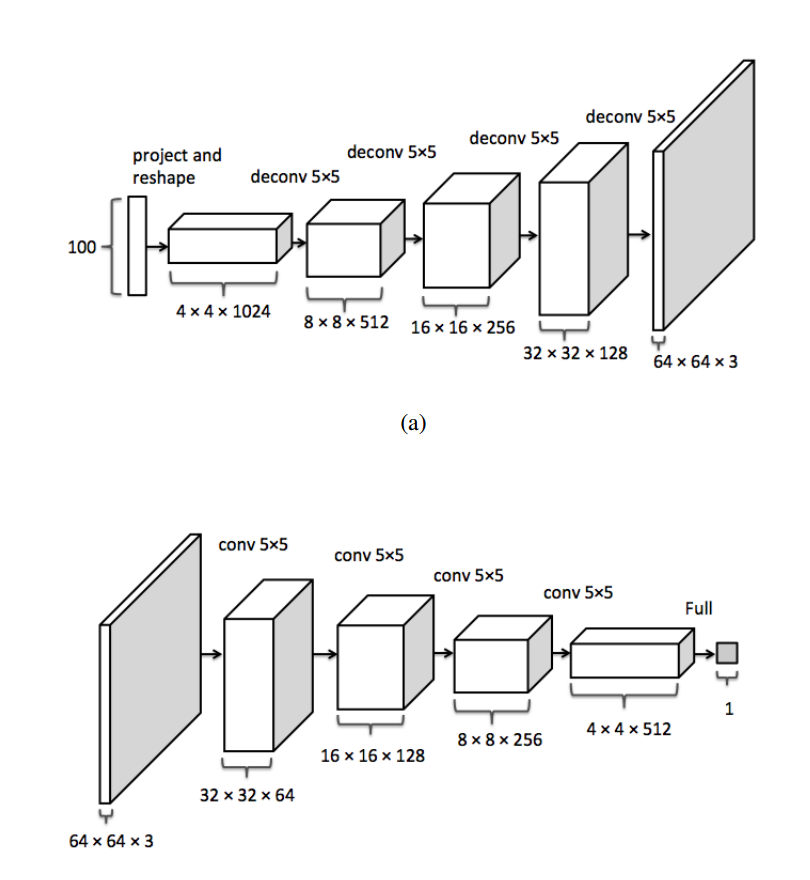
\includegraphics[scale=.3, angle=0]{Files/DCGAN.png}
    \caption[Generator and Discriminator  Architecture]{Generator and Discriminator Architecture\cite{DCGAN}}
    \label{fig:DCGAN}
\end{figure}

\begin{figure}[H]
  \centering
    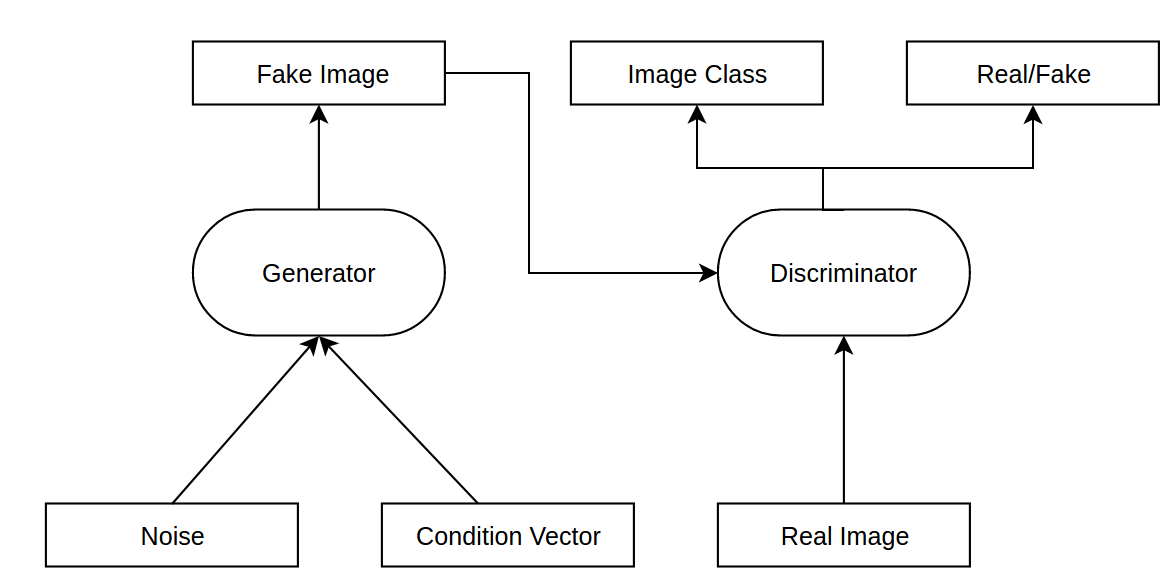
\includegraphics[scale=.3, angle=0]{Files/cgan.png}
    \caption[Conditional Generative Adversarial Network]{Conditional Generative Adversarial Network}
    \label{fig:CGAN}
\end{figure}
By looking at the architecture of the generator and discriminator in \cref{fig:DCGAN}, we will notice that they are  opposite to each other. The generator uses up-convolution or commonly known as backward convolution to generate images, whereas %J. Long, E. Shelhamer, and T. Darrell, “Fully convolutional networks for semantic segmentation,”CoRR, vol. abs/1411.4038, 2014. [Online]. Available: http://arxiv.org/abs/1411.4038
the discriminator is a standard deep convolution neural network used for classification of a real or a fake image.

The major contribution of DCGAN in our work is the use of Batch-Normalization, Strided Convolution and ADAM optimizer. We will go through each of these steps one by one.
\subsection{Batch Normalization}

Batch Normalization was first introduced by Ioffe  \textit{et al.} \cite{BatchNorm}. It was a major landmark in the area of deep learning as most of the current deep neural network frameworks contained batch normalization. 
To understand batch normalization, we need to understand the problem it is trying to solve. Its major aim is to minimize internal co-variance shift which refers to the change in input distribution as we are feed data in mini batches. Since neural networks are designed in a hierarchical fashion, even small changes in the form of an outlier can get amplified, as we are dealing with generally more than a million parameters and several layers. To rectify this problem, we normalize each batch at every layer, by both mean and variance. This process is commonly called whitening. The two major advantages of batch normalization are:
\begin{itemize}
    \item Initial values of weights have less impact on gradient descent.
    \item It helps in keeping higher learning rate and accuracy, hence reduces overall training time and helps in faster training of the GANs.
\end{itemize}

\subsection{Strided Convolution}

The concept of deconvolution was first introduced by Zeiler \textit{et al} \cite{Deconv}. It is also commonly known as  strided convolution, transposed fractional convolution, or upsampling. The idea is to go from the output of a convolution to the input of that convolution. For instance, it is going from the green matrix which is a convolution kernel to the blue matrix as shown in the below \cref{fig: Strided Convolution}. So given a kernel K, the type of convolution is defined by how forward or backward passes are calculated \cite{Deconv-Theano}.


\begin{figure}[H]
  \centering
    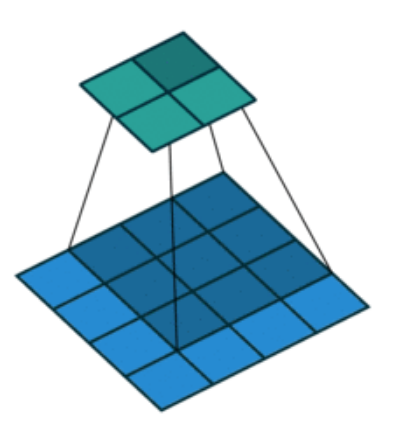
\includegraphics[scale=.4, angle=0]{Files/simple-conv.png}
    \caption[Simple Convolution]{Simple Convolution \cite{Deconv-Theano}}
    \label{fig: Simple Convolution}
\end{figure}
\begin{figure}[H]
  \centering
    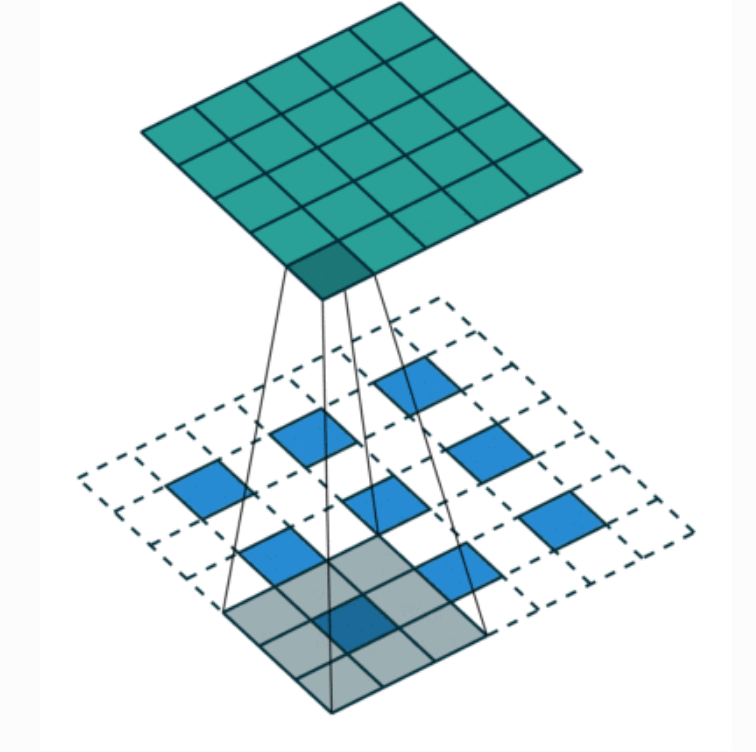
\includegraphics[scale=.3, angle=0]{Files/Frational-Stride-Conv.png}
    \caption[Transpose Convolution ]{Transpose Convolution \cite{Deconv-Theano}}
    \label{fig: Strided Convolution}
\end{figure}



\subsection{ADAM Optimizer}

Adaptive Moment Estimation, commonly known as ADAM is a stochastic gradient descent (SGD) optimizer. It was first proposed by Diederik \textit{et al.} \cite{Adam}. The vanilla stochastic gradient descent suffers from many problems. The three key issues which are directly related to our work are as follows:
\begin{itemize}
    \item In the case of non convex error functions, the neural network can be stuck in non local optima.
    \item Choosing correct learning rate is always a challenging task and can cause longer time for SGD algorithm to converge.
    \item Specifically in our work, where we are trying to model the data and it is sparse, Vanilla SGD does not provide flexibility for having different learning rates for each weight.

To overcome these problems, we use the ADAM optimizer in our work. It combines Adagrade \cite{Adagrade} and momentum-optimizer\cite{momentum} by storing not only exponentially decaying average of past squared gradients, but also keeping potentially decaying averages of past gradients $m_t$. The general steps of updating parameters using ADAM optimizer are as follows :
\begin{itemize}
    \item Initialize step size $\alpha$ and exponential decay parameters $\beta_1, \beta_2  \in [\![ 0,1]\!]$
    \item Compute gradient $g_t$ at current time t.
    \item Compute the first $m_t$ and second moment $v_t$.
    \begin{equation}\label{eq:moment}
        \begin{aligned}
            m_t = \beta_1 \times m_{t-1} + \left ( 1 - \beta_1 \right ) \times g_t \\
            v_t= \beta_2 \times v_{t-1} + \left ( 1 - \beta_2 \right ) \times g_t^{2}
        \end{aligned}
    \end{equation}
    \item Compute bias-corrected first  and second moment estimates.
     \begin{equation}\label{eq:moment2}
        \begin{aligned}
            \widehat{m}_t = \frac{m_t}{1-{\beta_1}^{t}} \\
            \widehat{v}_t = \frac{v_t}{1-{\beta_2}^{t}}
        \end{aligned}
    \end{equation}
    \item Now update the parameters $\theta_t$.
    \begin{equation}\label{eq:moment3}
        \begin{aligned}
            \theta_t =\theta_{t-1} - \alpha \times \frac{\widehat{m_{t}}}{\sqrt{\widehat{v_t} + \epsilon }}
        \end{aligned}
    \end{equation}
\end{itemize}

\end{itemize}
 